\chapter{Individual differences in reading and their relationship to intrinsic network architecture}

\section{Motivation}

First, we would like to establish what, if any, relationship intrinsic network architecture has with individual differences in reading. There is clear support for this idea in the literature: whole-brain measures of architecture have correlated with intelligence and psychiatric disorders. However, reading presents a unique opportunity to focus on a variety of skills. 

In particular, we are interested in whether this might be apparent through resting-state fMRI, which can be performed before children even start reading. As shown in the literature, we expect to see increases in ``intrinsic'' connectivity between secondary visual processing areas and language areas; however, the ``parasitic'' model would suggest that there would also be increased connectivity between the visual network and other systems throughout development and in better readers. 

\begin{itemize}
    \item First, we validate the existence of a small-world architecture in these subjects, and that the network parcellation is appropriate for them.
    \item Second, we determine whether global measures of interconnectedness, including modularity, participation coefficient and path length, are related to reading skill.
    \item Finally, we investigate which resting-state networks or brain regions drive the relationship between connectivity and reading skill.
\end{itemize}


\section{Methods}

The following methods detail the current study's protocol and analytic approach. The following chapters borrow heavily from the methods described below, so they are explained here in detail. 

\subsection{Participants}

Participants were drawn from the fourth wave of a larger, longitudinal study investigating the neurobiological bases of reading comprehension. 52 children completed scans and a subset of these met the motion and attention thresholds described below.

All participants were native English speakers with normal hearing and normal or corrected vision, and no history of major psychiatric illness or traumatic brain injury/epilepsy. Subjects had no history of a developmental disability or contra-indication to MRI.  Each participant gave written consent at the beginning of the study, with procedures carried out in accordance with Vanderbilt University’s Institutional Review Board.

\begin{table}
    \renewcommand{\tabcolsep}{0.09cm}
    \centering
    \begin{tabular}{lc}
\toprule 
Measure & Subjects \\ 
\midrule 
No. Participants				& 42 \\ 
No. Scan Runs					& 164 \\ 
Gender  						& 25 F \\ 
Age at Scan 					& 10.5 (0.3)  \\ 
WASI Full-Scale IQ  			& 111.0 (16.2) \\ 
TOWRE - Total Word Efficiency 	& 104.6 (18.5) \\ 
\bottomrule 
\end{tabular}
    \caption[Participant demographics]{Demographics and mean test scores for Study 1 participants are described here. For continuous data, the standard deviation is enclosed in parentheses.}
    \label{table:ch2-participants}
\end{table}

In addition to having an MRI scan, participants completed cognitive tests, including the Wechsler Abbreviated Scale of Intelligence (WASI) \citep{Kaplan1999}, the Test of Word Reading Efficiency (TOWRE) \citep{Torgesen2012}, the Woodcock Reading Master Tests (WRMT) \citep{Woodcock1998}, and the Gates-MacGinitie Reading Comprehension test \citep{MacGinitie2000}. Demographics and selected test data are summarized in Table \ref{table:ch2-participants}.

\subsection{MRI acquisition and preprocessing}

Imaging was performed on a Philips Achieva 3T MR scanner with a 32-channel head coil. Functional images were acquired using a gradient echo planar imaging sequence with 40 (3 mm thick) slices with no gap. Resting-state fMRI scans consisted of 150 dynamic volumes. Slices were parallel to the anterior-posterior commissure plane. Imaging parameters for functional images included: TE = 30 ms; FOV = 240 x 240 x 120 mm\textsuperscript{3}; flip angle = 75\degree; TR = 2200 ms; and 3 mm\textsuperscript{3} isotropic voxels.

\begin{figure}[t]
    \centering
    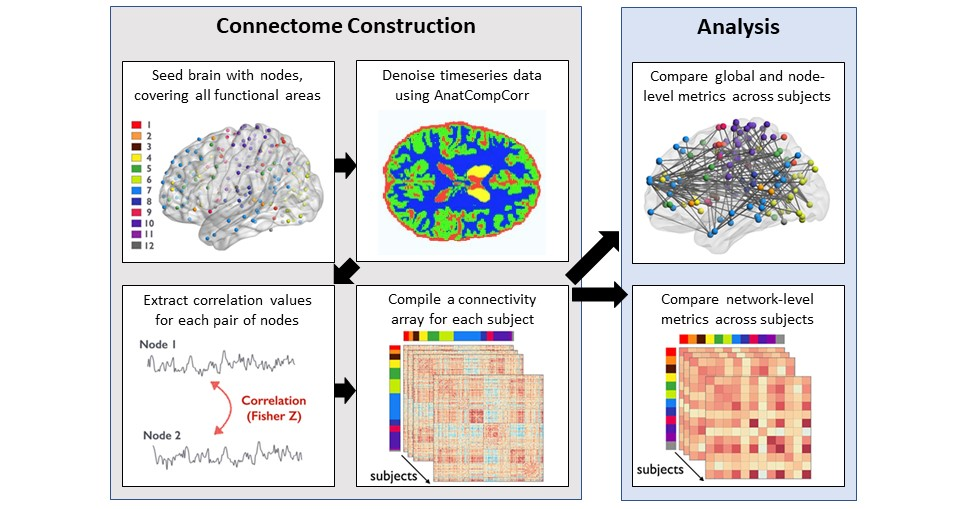
\includegraphics[width=6in]{ch2-connectome-methods}
    \caption[Schematic for connectome construction.]{Connectomes are constructed from resting-state fMRI in the following steps: slice-timing correction, rigid-body motion correction, boundary-based registration to a T1-weighted anatomical image, and normalization to MNI 152 template. The timseries for 264 nodes are then extracted and denoised using signal from non-neural tissue, continuous motion parameters and outliers. A pair-wise connectivity matrix is then calculated and thresholded at multiple different thresholds, then analyzed. Figure adapted from \citep{Yang2018}.}
    \label{fig:ch2-connectome-methods}
\end{figure}

Whole-brain fMRI analyses were performed using tools from the FMRIB Software Library (version 5.0.9). For each session, the following pre-processing steps were performed:  slice-time correction, motion correction to the initial fMRI volume, boundary-based registration to the subject's structural image, and normalization to 2 mm MNI 152 standard space. To mitigate the effects of motion on our analyses, we regressed out 6 continuous motion parameters and scrubbed out outlier volumes. We defined an outlier volume as any in which the root-mean-square framewise displacement exceeded 0.7 mm. Because head motion can be a major confound for connectivity analyses, we removed scan runs where more than 20 percent of the fMRI volumes were outliers.

\subsection{Connectome construction}

To investigate whole-brain patterns of connectivity with minimal investigator bias, we selected 264 nodes \textit{a priori} whose connectivity properties have been extensively analyzed in previous works \citep{Power2011}. The node set samples the entire brain, and nodes were selected based on their involvement in a diversity of cognitive tasks. Each node was assigned to one of 13 RSNs based on previous literature \citep{Power2013}. Approximately 10 percent of the nodes did not have a stable assignment in the original paper; for the present analyses, these nodes were excluded from graph theory calculations. A description of the 13 networks and their sizes is provided in \ref{table:ch2-power-nodes}. 

\begin{table}
	\renewcommand{\tabcolsep}{0.09cm}
	\centering
	\begin{tabular}{lcc}
\toprule 
Suggested RSN & Abbreviation & Nodes \\ 
\midrule 
\textit{Sensory} & & \\
	\hspace{3pt}Auditory  			&  AUD & 13 \\ 
	\hspace{3pt}Somatomotor (Hand)	&  SOH & 30 \\
	\hspace{3pt}Somatomotor (Mouth)	&  SOM & 5 \\
	\hspace{3pt}Visual	 			&  VIS & 31 \\ 
\textit{Attention} & & \\
	\hspace{3pt}Dorsal attention  	&  DAN & 11	\\ 
	\hspace{3pt}Salience		  	&  SAL & 18 \\ 
	\hspace{3pt}Ventral attention  	&  VAN & 9 \\ 
\textit{Executive / Associative} & & \\
	\hspace{3pt}Cingulo-opercular 	& CON & 14 \\ 
	\hspace{3pt}Default mode		& DMN & 58 \\
	\hspace{3pt}Fronto-parietal  	& FPN & 25 \\ 
	\hspace{3pt}Memory retrieval	& MEM & 5 \\
\textit{Other} & & \\
	\hspace{3pt}Cerebellar			& CER & 4  \\
	\hspace{3pt}Subcortical			& SUB & 13 \\
	\hspace{3pt}Not assigned 		& UNC & 28 \\ 
\bottomrule 
\end{tabular}
	\caption[List of networks.]{List of networks used in connectivity analyses and the number of nodes affiliated with each. Although alternative parcellations of the node set are possible, we elected to use those network assignments suggested in \citep{Power2013}.}
	\label{table:ch2-power-nodes}
\end{table}

Connectivity analysis was performed in the CONN toolbox \citep{WhitfieldGabrieli2012}. fMRI data were high-pass filtered at 0.008 Hz, motion-corrected, co-registered to a structural image, normalized to MNI space and smoothed by a 5 mm FWHM spherical kernel. Outlier volumes were identified as individual fMRI volumes in which the RMS framewise-displacement exceeded 0.7. fMRI timeseries were corrected using anatCompCorr methods, which uses signal from white matter tissue and cerebrospinal fluid areas to reduce noise not related to brain activity \citep{Chai2012}. We also regressed out 12 continuous measures of motion were also included and all outlier timepoints. The timeseries was then high-pass filtered at 0.01 Hz. fMRI timeseries correlations were calculated between each of the the 264 nodes, resulting in a single connectivity array for each subject at each time point. Matrices were then thresholded into binary maps by keeping the top 5 percent of connections. (To confirm that this particular threshold did not unduly influence results, we swept results between thresholds at the top 2 percent to the top 10 percent of connections. No significant effect on the results was found.)

\subsection{Connectome analyses}

The metrics of interest were network \textit{modularity}, \textit{participation coefficient} and \textit{path length}. Modularity is high in networks where nodes within the same RSN are highly connected to each other but not elsewhere. The participation coefficient, on the other hand, is high when many nodes are connected to several different RSNs. Both of these metrics relate to the integration of information between RSNs. Path length describes the distance between any two nodes on the graph. This was calculated between every node, then summed up by RSN to create a measure of network distance. These properties, and their changes within our task, were investigated at the level of connectomes, RSNs and nodes. 

First, we establish the validity of the parcellation for evaluting network properties in this sample. At rest, we expect to see high modularity (greater than 0.1), low participation (less than 0.9), and a lower path length within RSNs than between them. We also expect to see moderate-sized correlations between measures, since each is measuring an aspect of network architecture related to distance between nodes.  

Next, we break each global measure down by RSN to determine how sub-systems differ in their network roles. For modularity, we report the total modularity contribution for each network. For participation coefficient and path length, we report the mean value within each network. We also investigate the measures obtained across the whole range of network-forming thresholds (retaining the top 2 to 10 percent of connections). We expect to see changes in the measures across thresholds, but ranked in a relatively stable order among the different RSNs. 

To determine the relationship between network measures and individual performance on cognitive assessments, we input each global metric into a general linear model with the Test of Word Reading Efficiency (TOWRE, total word efficiency (TWE) standard score). Models containing measures of mean framewise-displacement (motion) and the WASI Vocabulary measure were also assesed to ensure that effects were not driven by motion confounds or global measures of cognitive skill. We also examined whether there were differences in the modularity relationship between TOWRE subtests (sight word efficiency (SWE) and phonemic decoding efficiency (PDE)). 

To assess whether there was an RSN-level trend in the modularity-to-reading relationship, post-hoc analyses comparing network-level modularity values to TOWRE scores were also investigated. For each node, a correlation value was calculated between its modularity contribution and TOWRE TWE scores. To evaluate significance, RSN correlations were compared to a bootstrapped distribution of 5000 correlation values generated by sampling and totaling the modularities for a random set of nodes equal in size to the selected RSN. (For example, adding 31 random nodes for comparison to the visual network.)


\section{Results} 

Of the 52 subjects who completed resting-state fMRI scans, 44 met the scan quality criteria for inclusion. Connectome parcellations at the 5 percent threshold exhibited small-world properties: the mean modularity value was 0.264 (SD = 0.037), and the mean participation coefficient was 0.599 (0.052). Furthermore, the path length within RSNs was significantly lower than those between: within-community nodes took an average of 2.49 (0.141) steps to reach each other, whereas between-community nodes took an average of 3.06 (0.207) steps ($p$ \textless 0.001, two-sample $t$-test). Furthermore, a comparison of each metric against the others shows that, while there is overlap between the measures at the global level, there is substantial variability as well (Table \ref{fig:ch2-global-graph-theory-descriptions}).

\begin{figure}[t]
    \centering
    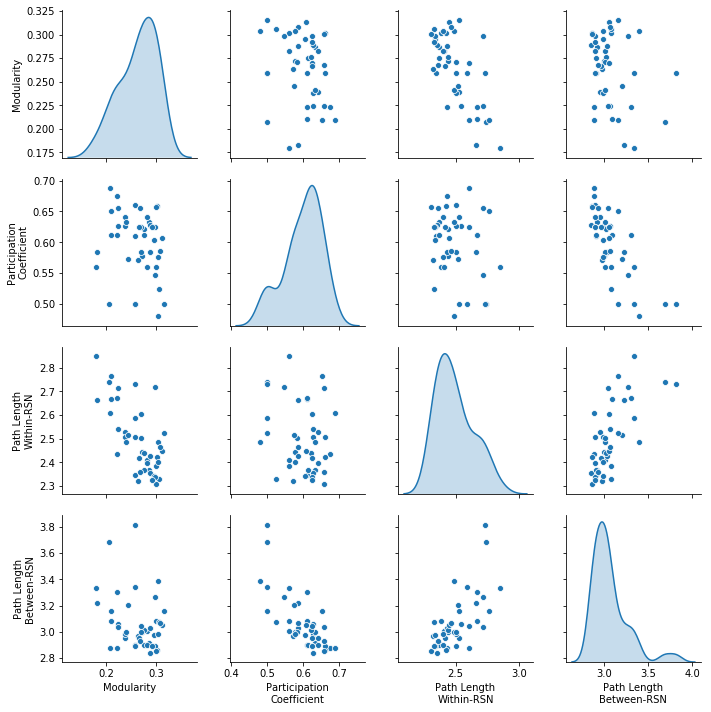
\includegraphics[width=5in]{ch2-global-graph-theory-descriptions}
    \caption[Distribution and correlations between global graph theory measures.]{Distribution and correlations between the global modularity, participation coefficient and path length. Each attribute may be interpreted as a measure of connectedness between RSNs, but there is significant variability between them.}
    \label{fig:ch2-global-graph-theory-descriptions}
\end{figure}

Comparing the contributions of each RSN to these global metrics highlights important differences between them.
- Visual, somatomotor, default mode and front-porietal networks were highest in modularity. 
- the FPN was interesting in theat it had higher modularity, moderate participation coefficient and lower path length
- loosening the threshold decreased modularity, increased participation coefficient and decreased path length.
- 5 percent is optimal for differences.
% try tsplot on bottom


\begin{figure}[t]
    \centering
    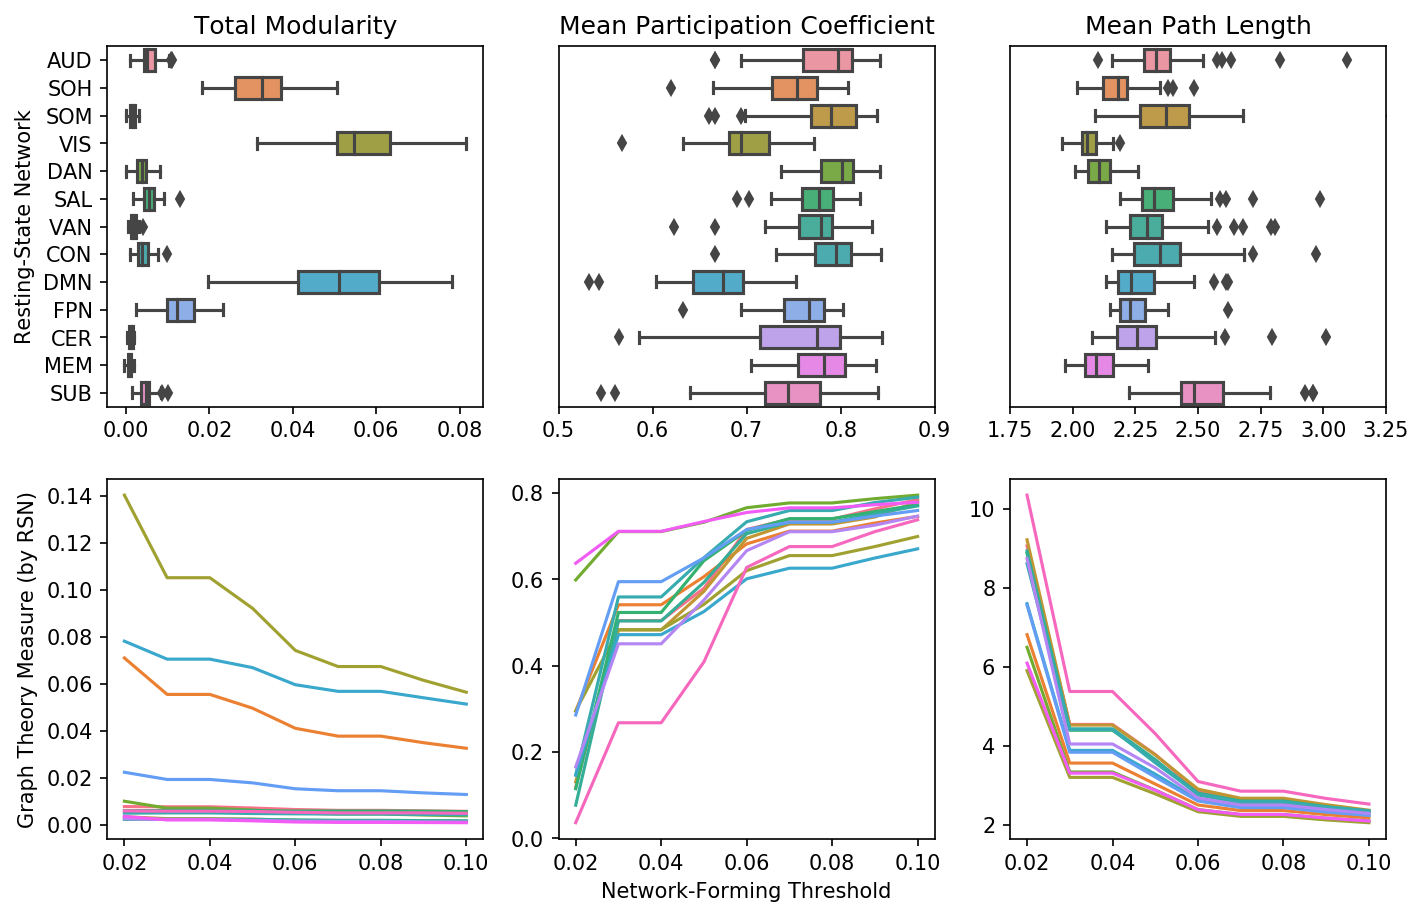
\includegraphics[width=6.1in]{ch2-network-graph-theory-descriptions}
    \caption[Relationships between network-level graph theory measures.]{Relationships between network-level graph theory measures. Each RSN plays a unique role in bridging areas of the brain. Shown above are the network-level distributions of the graph theory measures when graphs are thresholded for the top 10 percent of connections (top row), and the network means as the network-forming thresholds are swept from 2 percent to 10 percent (bottom row).}
    \label{fig:ch2-network-graph-theory-descriptions}
\end{figure}

\begin{table}[t]
    \renewcommand{\tabcolsep}{0.09cm}
    \centering
    \begin{tabular}{lcc}
\toprule 
Independent Variable & Coeff. & $p$-value \\ 
\midrule 
\textit{Sensory} & & \\
	\hspace{3pt}Auditory  			&  AUD & 13 \\ 
	\hspace{3pt}Somatomotor (Hand)	&  SOH & 30 \\
	\hspace{3pt}Somatomotor (Mouth)	&  SOM & 5 \\
	\hspace{3pt}Visual	 			&  VIS & 31 \\ 
\textit{Attention} & & \\
	\hspace{3pt}Dorsal attention  	&  DAN & 11	\\ 
	\hspace{3pt}Salience		  	&  SAL & 18 \\ 
	\hspace{3pt}Ventral attention  	&  VAN & 9 \\ 
\textit{Executive} & & \\
	\hspace{3pt}Cingulo-opercular 	& CON & 14 \\ 
	\hspace{3pt}Default mode		& DMN & 58 \\
	\hspace{3pt}Fronto-parietal  	& FPN & 25 \\ 
	\hspace{3pt}Memory retrieval	& MEM & 5 \\
\textit{Other} & & \\
	\hspace{3pt}Cerebellar			& CER & 4  \\
	\hspace{3pt}Subcortical			& SUB & 13 \\
	\hspace{3pt}Not assigned 		& UNC & 28 \\ 
\bottomrule 
\end{tabular}
    \caption{Results for analyses comparing global graph theory metrics to reading skill.}
    \label{table:ch2-global-glm-results}
\end{table}

\begin{figure}[t]
    \centering
    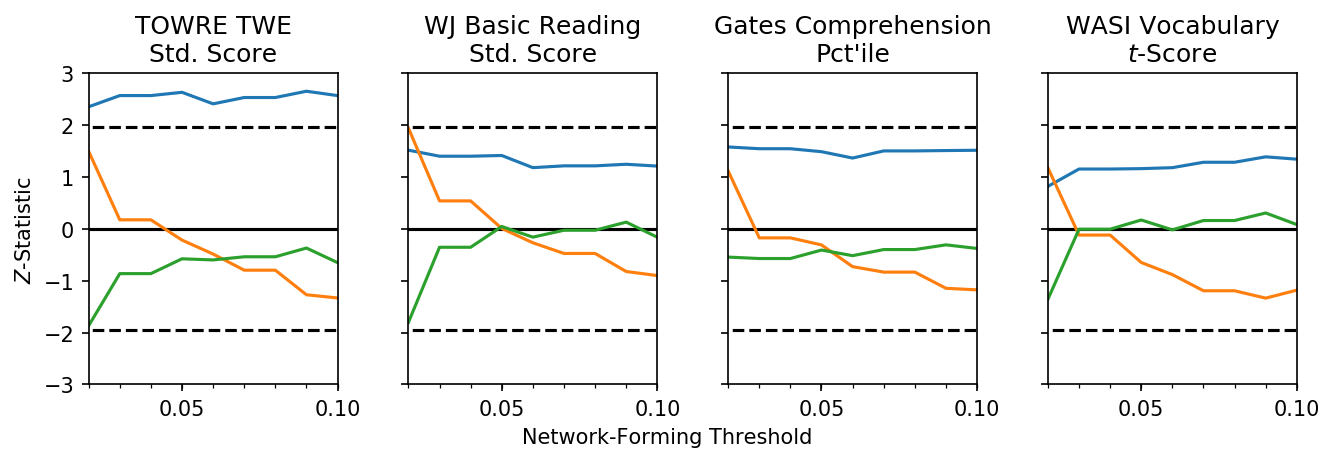
\includegraphics[width=5.5in]{ch2-global-glm-covariates-thresholds}
    \caption[Modularity metrics at rest are the best predictors of cognitive skills.] {Global modularity, the degree to which a whole-brain network separates into RSNs, was positively related to reading skill across all subjects ($N = 44$). Modularity for individual nodes was also positive overall ($r_{avg} = 0.134$), but was significantly higher for nodes in the visual, default mode and cingulo-opercular RSNs ($p < 0.01$). RSN colors correspond to the dominant Yeo RSN displayed in Fig. 1.}
    \label{fig:ch2-global-glm-covariates-thresh}
\end{figure}

\begin{figure}[t]
    \centering
    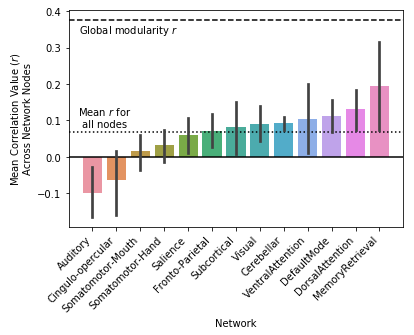
\includegraphics[height=3in]{ch2-rsn-node-modularity-corr}
    \caption[Modularity metrics at rest predict reading skill.] {Global modularity, the degree to which a whole-brain network separates into RSNs, was positively related to reading skill across all subjects ($N = 44$). Modularity for individual nodes was also positive overall ($r_{avg} = 0.134$), but was significantly higher for nodes in the visual, default mode and cingulo-opercular RSNs ($p < 0.01$). RSN colors correspond to the dominant Yeo RSN displayed in Fig. 1.}
    \label{fig:ch2-rsn-node-modularity-corr}
\end{figure}


Individual differences in global modularity were predictive of TOWRE - Total Word Efficiency standard scores. Modularity had a significant positive relationship with out-of-scanner reading metrics (for all subjects: $r = 0.299$, $p = 0.013$). This effect was also significant when data was analyzed separately by grade ($r_{G3} = 0.333$, $p = 0.014$; $r_{G4} = 0.359$, $p = 0.012$). The two subtests that constitute the TOWRE both showed a positive relationship with global modularity, as well ($r_{PDE} = 0.314$, $p = 0.009$; $r_{SWE} = 0.251$, $p = 0.039$). 

When examined at the individual node level, the average correlation between modularity and TOWRE scores was 0.134. Three RSNs had average node correlations that were significantly higher than this global network mean: the default mode ($r = 0.183$, $p$ \textless $0.001$), visual ($r = 0.183$, $p = 0.004$) and cingulo-opercular networks ($r = 0.224$, $p$ \textless $0.001$) (Fig. 2B). 

\section{Discussion}

In this first section, we establish that resting-state fMRI can connect robustly to behavioral metrics of reading efficiency. Modularity, in particular, indexes these skills. This is consistent with previosu research: the degree of segregation is critically important at rest. 

The distribution of the modularity is equally important: we see theat certain networks provide a larger aomuont of modularity per node than others. 

How the connectome changes during reading is an important next step that we will tackle in the following chapter.